\documentclass[12pt]{kupaper}
%プリアンブルの読み込み
\input{./documents/preamble.tex}
%マクロ定義した数式の読み込み
\input{./documents/define_equations.tex}

\begin{document}
%%% includeはできるだけつかわないでください!!

%論文タイトル
\Title{論文執筆要領}
%論文著者
\Author{橋本 勇輝}
%指導教員
\Professor{馬塲 一晴}
%学籍番号
\StudentNumber{212270040}
%提出日
\Date{6}%2022 卒論用
\Date{6}%2023 修論用
%英語用なので以下は無視して良い.ただし消さないように.
\title{How to write a master's thesis}
\author{Yuki Hashimoto}
\professor{Kazuharu Bamba}
\endate{February}{15}{2025} %2022 卒論用
\endate{February}{2}{2025}  %2023 修論用

%学部の人は次のコメント行の%を外してください.
%\senior
%この\seniorは\Abstractの前であればどこに書いてもかまいません.

\Maketitle

%\setcounter{chapter}{20}
% 目次  (LaTeX の処理を少くする目的で,最後に書いています)
\pagenumbering{roman}
\setcounter{page}{1}
\tableofcontents

\begin{comment} %必要に応じて利用してください.
\clearpage
\listoffigures
\clearpage
\listoftables
\end{comment}

\chapter{序論}
\pagenumbering{arabic} % 絶対必要です.最初の章にのみ記述します.

卒業論文・修士論文は,みなさんのこれまでの研究の成果をまとめて報告し,みなさんがそれぞれの学位に値するかを審査するための重要な論文です.そのためには,これまでの研究成果の内容をよく吟味し,「人に自分の考えを伝える」重要性と難しさに注意し,分かりやすい表現を考え,書いた文章をよく推敲し,さらに,論文として定められた形式をとる必要があります.

\chapter{\LaTeX の基本}
\section{参考文献の引用方法}
参考文献を論文中で引用するときはref.bibファイルに参考文献情報を貼り付けたうえで次のように引用しましょう\cite{G_ng_r_2021}.
\section{数式について}
文中式は $\hat{g}_{\mu\nu}=e^{2\omega}g_{\mu\nu}$ と書けます.その他別行立ての数式は次のような数式環境を用いて入力します.

よく使用する数式については,./documents/define\_equations.texに,newcommandでマクロを定義しておくと便利です.
	\begin{equation}
		R_{\mu\alpha\nu}^{\lambda}=\Riemanntensor{\lambda}{\mu}{\alpha}{\nu}{\sigma}\label{eq:Riemann_tensor}
	\end{equation}

また,複数行にわたる数式変形をきれいに出力したいときは,dmath環境を用いると便利です.dmath環境では数式を自動で改行したり,等号の位置を自動で揃えてくれます.
	\begin{dmath}
		R_{rr} = \partial_{\lambda}\chr{\lambda}{r}{r}
		- \partial_{r}\chr{\lambda}{\lambda}{r}
		+ \chr{\lambda}{\lambda}{\ell}\chr{\ell}{r}{r}
		- \chr{\lambda}{r}{\ell}\chr{\ell}{\lambda}{r}
		= \qty{\partial_{t}\chr{t}{r}{r} - \partial_{r}\chr{t}{t}{r} + \chr{t}{t}{\ell}\chr{\ell}{r}{r} - \chr{t}{r}{\ell}\chr{\ell}{t}{r}}
		+ \qty{\partial_{\theta}\chr{\theta}{r}{r} - \partial_{r}\chr{\theta}{\theta}{r} + \chr{\theta}{\theta}{\ell}\chr{\ell}{r}{r} - \chr{\theta}{r}{\ell}\chr{\ell}{\theta}{r}}
		+ \qty{\partial_{\varphi}\chr{\varphi}{r}{r} - \partial_{r}\chr{\varphi}{\varphi}{r} + \chr{\varphi}{\varphi}{\ell}\chr{\ell}{r}{r} - \chr{\varphi}{r}{\ell}\chr{\ell}{\varphi}{r}} \nonumber \\
		= \qty{\partial_{t}\chr{t}{r}{r} - \chr{t}{r}{r}\chr{r}{t}{r}}
		+ \qty{- \partial_{r}\chr{\theta}{\theta}{r} + \chr{\theta}{\theta}{t}\chr{t}{r}{r} + \chr{\theta}{\theta}{r}\chr{r}{r}{r} - \chr{\theta}{r}{\theta}\chr{\theta}{\theta}{r}}
		+ \qty{- \partial_{r}\chr{\varphi}{\varphi}{r} + \chr{\varphi}{\varphi}{t}\chr{t}{r}{r} + \chr{\varphi}{\varphi}{r}\chr{r}{r}{r} - \chr{\varphi}{r}{\varphi}\chr{\varphi}{\varphi}{r}} \nonumber \\
		= \frac{\dot{a}^2+a\ddot a}{1-Kr^2} - \frac{a\dot a}{1-Kr^2}\frac{\dot a}{a} + \frac{1}{r^2} + \frac{\dot a}{a}\frac{a\dot a}{1-Kr^2} + \frac{1}{r}\frac{Kr}{1-Kr^2} + \frac{\dot a}{a}\frac{a\dot a}{1-Kr^2} + \frac{1}{r}\frac{Kr}{1-Kr^2} -\frac{1}{r^2} \nonumber \\
		= \frac{2\dot{a}^2+a\ddot a + 2K}{1-Kr^2}\label{eq:Ricci_tensor}
	\end{dmath}

  論文中の数式を引用したい場合は,引用したい数式にラベルを付け,引用したい箇所で「\textbackslash cref\{eq:作成したラベル\}」と入力すれば\cref{eq:Ricci_tensor}のように引用が可能です.数式ラベル内にeq:とつけているのは数式をエディタの検索機能や補完機能を利用しやすくするためです.

  その他,数式を入力する際には,physicsパッケージを用いるのが便利です(usepackageしてあります).

\section{図の挿入と引用}
図は以下のように挿入できます.
	\begin{figure}[htbp]
		\centering
		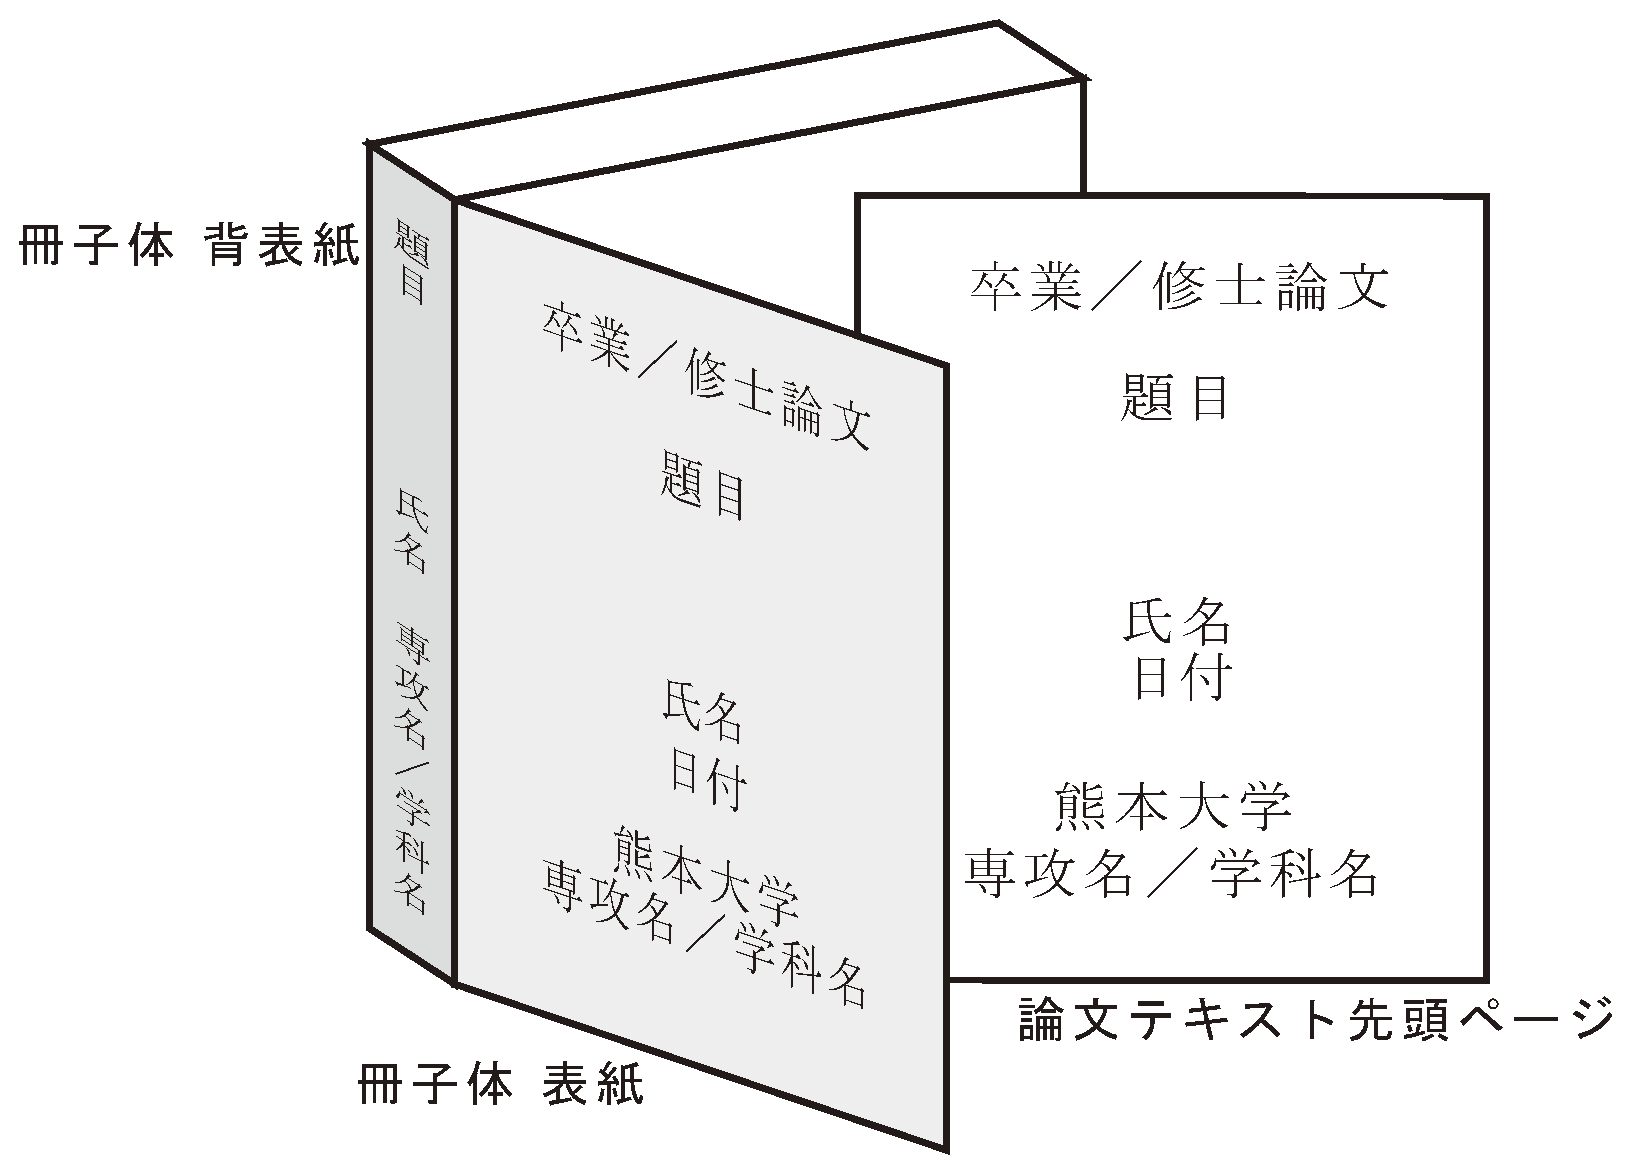
\includegraphics[width=1.0\linewidth,keepaspectratio]{./images/book.eps}
		\caption{冊子体および論文テキストの先頭ページ}
		\label{fig:overview}
	\end{figure}

また,文中の図を引用したい場合は,図にラベルを付けて\cref{fig:overview}としましょう.

\section{付録へのソースコードのつけ方}

付録にソースコードをつける場合,本テンプレートに付属の「jlisting.sty」を以下の手順で適切な場所に置く必要があります.

	\begin{enumerate}
		\item jlisting.sty をC:\textbackslash texlive \textbackslash texmf-local\textbackslash tex \textbackslash latex\textbackslash local \textbackslash listings ディレクトリに置く(listingsディレクトリがなければ作成).
		\item 管理者モードのコマンドプロンプトで「mktexlsr」と入力し実行.
	\end{enumerate}

これで問題なく実行できるはずです.

\chapter{メディアおよび必要部数}
	\begin{itemize}
		\item 卒業論文:冊子体1部および電子版 (PDFファイル)
		\item 修士論文:冊子体3部\footnote{論文審査委員が4名以上の場合は,その人数分の部数を準備すること.}および電子版 (PDFファイル)
	\end{itemize}

\chapter{提出先および投稿先}
提出可能時期については,各年度の執筆概要を参照してください.
	\begin{itemize}
		\item 冊子体:教務課,指導教員(修論は副査の先生方にも提出)
		\item 電子版:最終版を\href{https://forms.gle/ZUT2Erq8iPRBpF4q9}{卒論・修論提出フォーム}より提出.
	\end{itemize}

\chapter{冊子体の体裁}
表紙には,論文題目,学群,学類,コース,学籍番号,氏名,指導教員名,卒業年度が必要です.また,ページ番号は表紙以外のページ下中央に挿入しましょう.

\chapter{論文の構成}\label{chap:論文の構成}
論文は,以下の\crefrange{term:a}{term:f}の順序で構成してください.

	\begin{enumerate}[a.]
		\item 表紙 \label{term:a}
		\item 目次 \label{term:b}
		\item 本文 \label{term:c}
		\item 謝辞 \label{term:d}
		\item 付録 \label{term:e}
		\item 参考文献 \label{term:f}
	\end{enumerate}

\chapter{論文の記述要領}
	\begin{enumerate}[a.]
		\item 文書作成ソフトウェア等で作成してください.なお,電子版はPDF形式で投稿してください.
		\item 用紙のサイズはA4版とし,縦長・横書きを基本とします.
		\item \cref{chap:論文の構成} の\cref{term:a}にはページ番号を付けないでください.\cref{term:b}にはローマ数字の小文字 (i,ii,...) を使ってページ番号を付けてください.\crefrange{term:c}{term:f}は,アラビア数字 (1,2,...) を使って通しでページ番号を付けてください.
		\item ページ番号は本文の下中央部に記載してください.
		\item 文章は和文 (常用漢字・現代ひらがな) あるいは英文のいずれか一方で統一して書いてください.
		\item 術語は原則として各研究室に関連の深い学会の論文執筆基準に従ってください.また人名,書名,学会名等の固有名詞は,原語のまま用いてください.

			\begin{enumerate}[(例1)]
				\item
						分かりやすい簡潔な表現[5]を心掛けることは,論文執筆において重要なことである.\\
						{[5]} 木下是雄,「理科系の作文技術」,中央公論社 中公新書624,pp.118-152,1981.
				\item
						分かりやすい簡潔な表現(5)を心掛けることは,論文執筆において重要なことである.\\
						(5) 木下是雄,「理科系の作文技術」,中央公論社 中公新書624,pp.118-152,1981.
				\item \label{例3}
						分かりやすい簡潔な表現 (木下,1981) を心掛けることは,…
						(木下,1981)  \\
						木下是雄,「理科系の作文技術」,中央公論社 中公新書624,pp.118-152 1981.\\
						※(例3)の場合,参考文献リストは,著者のABC順に,同一著者は執筆年順に並べる.
			\end{enumerate}

		\item 図表等の番号と表題は,図や写真の場合には図や写真の下に,表の場合には表の上に記載します.
		\item その他のことについては,論文の書き方を説明した \cite{木下是雄2001理科系の作文技術,学術論文の書き方・発表の仕方,howtocite} のような文献を参考にしてください.\\

	\end{enumerate}

%謝辞
\begin{thanks}
	本論文を執筆するにあたり,感謝すべき人物,環境などがありましたら記述してください.
\end{thanks}

%付録(ソースコード)
\appendix
\chapter*{付録} % 章番号を出さない
\addcontentsline{toc}{chapter}{付録} % 目次に載せる

% 付録は chapter の 1 つとして作りますが、章番号は表示しません。
% また付録の 1 つずつはアルファベットで番号付けをするのが一般的です。
\setcounter{section}{0}% section の番号をゼロにリセットする
\renewcommand{\thesection}{\Alph{section}} % 数字ではなくアルファベットで数える
\setcounter{equation}{0}% 式番号を A.1 のようにする
\renewcommand{\theequation}{\Alph{section}.\arabic{equation}}
\setcounter{figure}{0}% 図番号
\renewcommand{\thefigure}{\Alph{section}.\arabic{figure}}
\setcounter{table}{0}% 表番号
\renewcommand{\thetable}{\Alph{section}.\arabic{table}}
\lstset{
  language = Python,
  %背景色と透過度
  backgroundcolor={\color[gray]{.90}},
  %枠外に行った時の自動改行
  breaklines = true,
  %自動改行後のインデント量(デフォルトでは20[pt])
  breakindent = 10pt,
  %標準の書体
  basicstyle = \ttfamily\scriptsize,
  %コメントの書体
  commentstyle = {\itshape \color[cmyk]{1,0.4,1,0}},
  %関数名等の色の設定
  classoffset = 0,
  %キーワード(int, ifなど)の書体
  keywordstyle = {\bfseries \color[cmyk]{0,1,0,0}},
  %表示する文字の書体
  stringstyle = {\ttfamily \color[rgb]{0,0,1}},
  %枠 "t"は上に線を記載, "T"は上に二重線を記載
  %他オプション:leftline,topline,bottomline,lines,single,shadowbox
  frame = TBrl,
  %frameまでの間隔(行番号とプログラムの間)
  framesep = 5pt,
  %行番号の位置
  numbers = left,
  %行番号の間隔
  stepnumber = 1,
  %行番号の書体
  numberstyle = \tiny,
  %タブの大きさ
  tabsize = 4,
  %キャプションの場所("tb"ならば上下両方に記載)
  captionpos = t
}

\section{数値解析コード}
ソースコード等を付録として示す場合は以下のようにしましょう.
%ソースコードのPathはmain.tex側から見た時のPathを指定
\lstinputlisting[caption = 使用した数値解析コード, label = program2]{./source_codes/source_code.py}

% 参考文献
\printbibliography[title=参考文献]
%\nocite{*}
\end{document}
